\documentclass[twoside]{article}

% Packages required by doxygen
\usepackage{calc}
\usepackage{doxygen}
\usepackage{graphicx}
\usepackage[utf8]{inputenc}
\usepackage{makeidx}
\usepackage{multicol}
\usepackage{multirow}
\usepackage{textcomp}
\usepackage[table]{xcolor}

% Font selection
\usepackage[T1]{fontenc}
\usepackage{mathptmx}
\usepackage[scaled=.90]{helvet}
\usepackage{courier}
\usepackage{amssymb}
\usepackage{sectsty}
\renewcommand{\familydefault}{\sfdefault}
\allsectionsfont{%
  \fontseries{bc}\selectfont%
  \color{darkgray}%
}
\renewcommand{\DoxyLabelFont}{%
  \fontseries{bc}\selectfont%
  \color{darkgray}%
}

% Page & text layout
\usepackage{geometry}
\geometry{%
  a4paper,%
  top=2.5cm,%
  bottom=2.5cm,%
  left=2.5cm,%
  right=2.5cm%
}
\tolerance=750
\hfuzz=15pt
\hbadness=750
\setlength{\emergencystretch}{15pt}
\setlength{\parindent}{0cm}
\setlength{\parskip}{0.2cm}
\makeatletter
\renewcommand{\paragraph}{%
  \@startsection{paragraph}{4}{0ex}{-1.0ex}{1.0ex}{%
    \normalfont\normalsize\bfseries\SS@parafont%
  }%
}
\renewcommand{\subparagraph}{%
  \@startsection{subparagraph}{5}{0ex}{-1.0ex}{1.0ex}{%
    \normalfont\normalsize\bfseries\SS@subparafont%
  }%
}
\makeatother

% Headers & footers
\usepackage{fancyhdr}
\pagestyle{fancyplain}
\fancyhead[LE]{\fancyplain{}{\bfseries\thepage}}
\fancyhead[CE]{\fancyplain{}{}}
\fancyhead[RE]{\fancyplain{}{\bfseries\leftmark}}
\fancyhead[LO]{\fancyplain{}{\bfseries\rightmark}}
\fancyhead[CO]{\fancyplain{}{}}
\fancyhead[RO]{\fancyplain{}{\bfseries\thepage}}
\fancyfoot[LE]{\fancyplain{}{}}
\fancyfoot[CE]{\fancyplain{}{}}
\fancyfoot[RE]{\fancyplain{}{\bfseries\scriptsize Generated on Sat Nov 9 2013 22\-:18\-:35 for Cat Mouse by Doxygen }}
\fancyfoot[LO]{\fancyplain{}{\bfseries\scriptsize Generated on Sat Nov 9 2013 22\-:18\-:35 for Cat Mouse by Doxygen }}
\fancyfoot[CO]{\fancyplain{}{}}
\fancyfoot[RO]{\fancyplain{}{}}
\renewcommand{\footrulewidth}{0.4pt}
\renewcommand{\sectionmark}[1]{%
  \markright{\thesection\ #1}%
}

% Indices & bibliography
\usepackage{natbib}
\usepackage[titles]{tocloft}
\setcounter{tocdepth}{3}
\setcounter{secnumdepth}{5}
\makeindex

% Custom commands
\newcommand{\clearemptydoublepage}{%
  \newpage{\pagestyle{empty}\cleardoublepage}%
}


%===== C O N T E N T S =====

\begin{document}

% Titlepage & ToC
\pagenumbering{roman}
\begin{titlepage}
\vspace*{7cm}
\begin{center}%
{\Large Cat Mouse \\[1ex]\large High Distinction Project for H\-I\-T2302 Object Oriented Programming }\\
\vspace*{1cm}
{\large Generated by Doxygen 1.8.5}\\
\vspace*{0.5cm}
{\small Sat Nov 9 2013 22:18:35}\\
\end{center}
\end{titlepage}
\tableofcontents
\pagenumbering{arabic}

%--- Begin generated contents ---
\section{Objective-\/\-C Coupled Implementation}
\label{index}\begin{DoxyVersion}{Version}
3 
\end{DoxyVersion}

\section{Class Documentation}
\subsection{C\-M\-Animal Class Reference}
\label{interface_c_m_animal}\index{C\-M\-Animal@{C\-M\-Animal}}


{\ttfamily \#import $<$C\-M\-Animal.\-h$>$}



Inheritance diagram for C\-M\-Animal\-:
\nopagebreak
\begin{figure}[H]
\begin{center}
\leavevmode
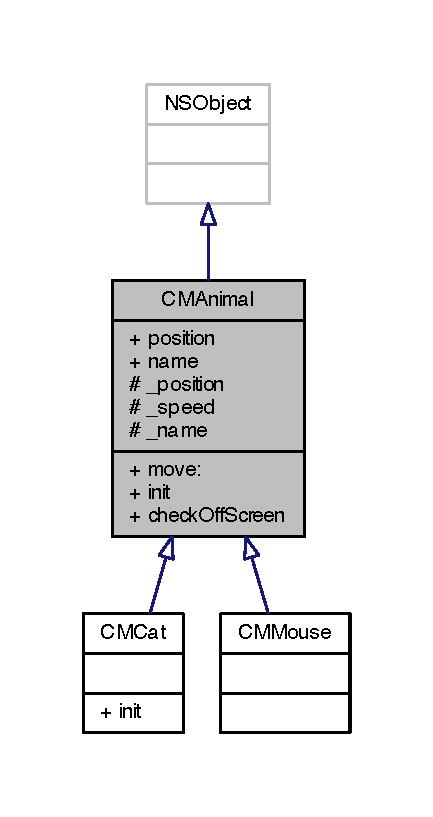
\includegraphics[width=208pt]{interface_c_m_animal__inherit__graph}
\end{center}
\end{figure}


Collaboration diagram for C\-M\-Animal\-:
\nopagebreak
\begin{figure}[H]
\begin{center}
\leavevmode
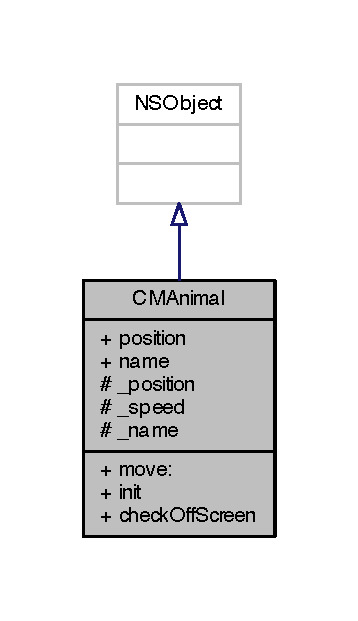
\includegraphics[width=172pt]{interface_c_m_animal__coll__graph}
\end{center}
\end{figure}
\subsubsection*{Instance Methods}
\begin{DoxyCompactItemize}
\item 
(void) -\/ {\bf move\-:}
\item 
(id) -\/ {\bf init}{\ttfamily  [implementation]}
\item 
(void) -\/ {\bf check\-Off\-Screen}{\ttfamily  [implementation]}
\end{DoxyCompactItemize}
\subsubsection*{Protected Attributes}
\begin{DoxyCompactItemize}
\item 
S\-G\-Point2\-D $\ast$ {\bf \-\_\-position}
\item 
int {\bf \-\_\-speed}
\item 
N\-S\-String $\ast$ {\bf \-\_\-name}
\end{DoxyCompactItemize}
\subsubsection*{Properties}
\begin{DoxyCompactItemize}
\item 
S\-G\-Point2\-D $\ast$ {\bf position}
\item 
N\-S\-String $\ast$ {\bf name}
\end{DoxyCompactItemize}


\subsubsection{Detailed Description}
Defines an abstract, base class for a playable `thing' on the screen which can move around etc. 

\begin{DoxyAuthor}{Author}
Alex Cummaudo 
\end{DoxyAuthor}
\begin{DoxyDate}{Date}
23 Oct 2013 
\end{DoxyDate}


\subsubsection{Method Documentation}
\index{C\-M\-Animal@{C\-M\-Animal}!move\-:@{move\-:}}
\index{move\-:@{move\-:}!CMAnimal@{C\-M\-Animal}}
\paragraph[{move\-:}]{\setlength{\rightskip}{0pt plus 5cm}-\/ (void) move\-: 
\begin{DoxyParamCaption}
\item[{({\bf dirs})}]{dir}
\end{DoxyParamCaption}
}\label{interface_c_m_animal_a0fa1cbfa194386482d87a3b817a5de7a}


Move implementation for a Animal to move an animal in a direction at its speed. 


\begin{DoxyParams}{Parameters}
{\em dir} & Direction the animal is told to move in (alters x and y axis position of poisition accordingly) \\
\hline
\end{DoxyParams}
\index{C\-M\-Animal@{C\-M\-Animal}!init@{init}}
\index{init@{init}!CMAnimal@{C\-M\-Animal}}
\paragraph[{init}]{\setlength{\rightskip}{0pt plus 5cm}-\/ (id) init 
\begin{DoxyParamCaption}
{}
\end{DoxyParamCaption}
\hspace{0.3cm}{\ttfamily [implementation]}}\label{interface_c_m_animal_a0c0294aa9117b8f382ccdd101725452c}


Default constructor for initialising \-\_\-position and \-\_\-speed for all new Animals. 

\begin{DoxyReturn}{Returns}
The self class pointer 
\end{DoxyReturn}


Reimplemented in {\bf C\-M\-Cat} \doxyref{}{p.}{interface_c_m_cat_a41400907a9f8aab9e36d9320f5a4db4b}.

\index{C\-M\-Animal@{C\-M\-Animal}!check\-Off\-Screen@{check\-Off\-Screen}}
\index{check\-Off\-Screen@{check\-Off\-Screen}!CMAnimal@{C\-M\-Animal}}
\paragraph[{check\-Off\-Screen}]{\setlength{\rightskip}{0pt plus 5cm}-\/ (void) check\-Off\-Screen 
\begin{DoxyParamCaption}
{}
\end{DoxyParamCaption}
\hspace{0.3cm}{\ttfamily [implementation]}}\label{interface_c_m_animal_af0f2f628a396447ba8854a07d24aedc1}


Off screen check that prevents any Animal from going outside the borders of the screen. 



\subsubsection{Member Data Documentation}
\index{C\-M\-Animal@{C\-M\-Animal}!\-\_\-position@{\-\_\-position}}
\index{\-\_\-position@{\-\_\-position}!CMAnimal@{C\-M\-Animal}}
\paragraph[{\-\_\-position}]{\setlength{\rightskip}{0pt plus 5cm}-\/ (S\-G\-Point2\-D$\ast$) \-\_\-position\hspace{0.3cm}{\ttfamily [protected]}}\label{interface_c_m_animal_ac54a37cee5d990bfdd897a29933f4c95}


Centrepoint position of the animal. 

\index{C\-M\-Animal@{C\-M\-Animal}!\-\_\-speed@{\-\_\-speed}}
\index{\-\_\-speed@{\-\_\-speed}!CMAnimal@{C\-M\-Animal}}
\paragraph[{\-\_\-speed}]{\setlength{\rightskip}{0pt plus 5cm}-\/ (int) \-\_\-speed\hspace{0.3cm}{\ttfamily [protected]}}\label{interface_c_m_animal_ad576084bf3f71ae6cb2d7429c2ab122d}


Speed at which animals move at, set to a value of 3. 

\index{C\-M\-Animal@{C\-M\-Animal}!\-\_\-name@{\-\_\-name}}
\index{\-\_\-name@{\-\_\-name}!CMAnimal@{C\-M\-Animal}}
\paragraph[{\-\_\-name}]{\setlength{\rightskip}{0pt plus 5cm}-\/ (N\-S\-String$\ast$) \-\_\-name\hspace{0.3cm}{\ttfamily [protected]}}\label{interface_c_m_animal_a7400051992ecd79e8d4bc9cd6d5c4e22}


Name of animals, overriden by children (i.\-e. `\-Cat' or `\-Mouse') 



\subsubsection{Property Documentation}
\index{C\-M\-Animal@{C\-M\-Animal}!position@{position}}
\index{position@{position}!CMAnimal@{C\-M\-Animal}}
\paragraph[{position}]{\setlength{\rightskip}{0pt plus 5cm}-\/ (S\-G\-Point2\-D$\ast$) position\hspace{0.3cm}{\ttfamily [read]}, {\ttfamily [write]}, {\ttfamily [atomic]}, {\ttfamily [retain]}}\label{interface_c_m_animal_a200958e5c164ccc76005cd3f6fcfc4de}


Readwrite property to update position, used by \doxyref{C\-M\-Game}{p.}{class_c_m_game}. 

\index{C\-M\-Animal@{C\-M\-Animal}!name@{name}}
\index{name@{name}!CMAnimal@{C\-M\-Animal}}
\paragraph[{name}]{\setlength{\rightskip}{0pt plus 5cm}-\/ (N\-S\-String$\ast$) name\hspace{0.3cm}{\ttfamily [read]}, {\ttfamily [atomic]}, {\ttfamily [assign]}}\label{interface_c_m_animal_ae04188fae2d235f67ef40a46181737c8}


Readonly property to name, used by \doxyref{C\-M\-G\-U\-I}{p.}{interface_c_m_g_u_i} and \doxyref{C\-M\-Network}{p.}{interface_c_m_network}. 



The documentation for this class was generated from the following files\-:\begin{DoxyCompactItemize}
\item 
/\-Users/\-Alex/\-Dropbox/\-Swinburne/\-H\-I\-T2302 -\/ O\-O\-P/\-Projects/\-Cat and Mouse/\#2\-\_\-\-Cat\-Mouse\-\_\-\-Obj\-C\-\_\-\-D\-E\-Coupled/src/{\bf C\-M\-Animal.\-h}\item 
/\-Users/\-Alex/\-Dropbox/\-Swinburne/\-H\-I\-T2302 -\/ O\-O\-P/\-Projects/\-Cat and Mouse/\#2\-\_\-\-Cat\-Mouse\-\_\-\-Obj\-C\-\_\-\-D\-E\-Coupled/src/{\bf C\-M\-Animal.\-m}\end{DoxyCompactItemize}

\subsection{C\-M\-Cat Class Reference}
\label{interface_c_m_cat}\index{C\-M\-Cat@{C\-M\-Cat}}


{\ttfamily \#import $<$C\-M\-Cat\-Mouse.\-h$>$}



Inheritance diagram for C\-M\-Cat\-:
\nopagebreak
\begin{figure}[H]
\begin{center}
\leavevmode
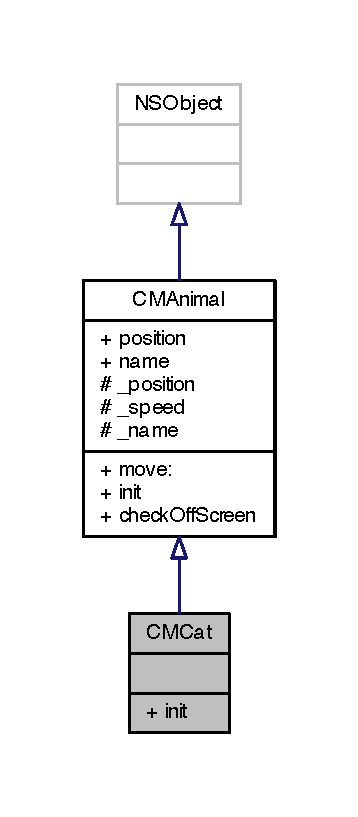
\includegraphics[width=172pt]{interface_c_m_cat__inherit__graph}
\end{center}
\end{figure}


Collaboration diagram for C\-M\-Cat\-:
\nopagebreak
\begin{figure}[H]
\begin{center}
\leavevmode
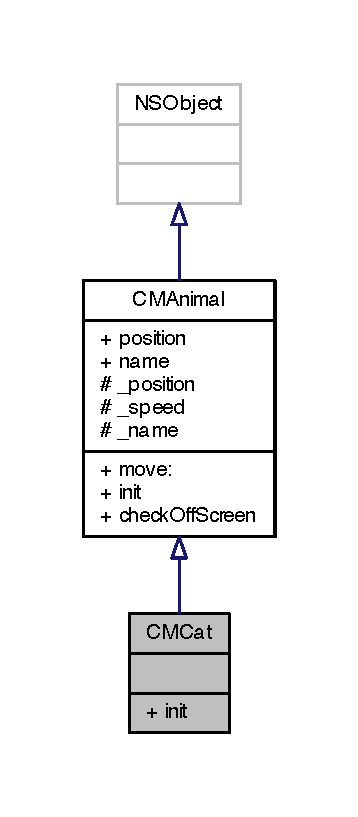
\includegraphics[width=172pt]{interface_c_m_cat__coll__graph}
\end{center}
\end{figure}
\subsubsection*{Instance Methods}
\begin{DoxyCompactItemize}
\item 
(id) -\/ {\bf init}{\ttfamily  [implementation]}
\end{DoxyCompactItemize}
\subsubsection*{Additional Inherited Members}


\subsubsection{Detailed Description}
Defines an class for a playable chaser (i.\-e. the chasing cat) 

\begin{DoxyAuthor}{Author}
Alex Cummaudo 
\end{DoxyAuthor}
\begin{DoxyDate}{Date}
24 Oct 2013 
\end{DoxyDate}


\subsubsection{Method Documentation}
\index{C\-M\-Cat@{C\-M\-Cat}!init@{init}}
\index{init@{init}!CMCat@{C\-M\-Cat}}
\paragraph[{init}]{\setlength{\rightskip}{0pt plus 5cm}-\/ (id) init 
\begin{DoxyParamCaption}
{}
\end{DoxyParamCaption}
\hspace{0.3cm}{\ttfamily [implementation]}}\label{interface_c_m_cat_a41400907a9f8aab9e36d9320f5a4db4b}


The default constructor for the cat constructs parent and sets position on lefthand-\/side of screen. 

\begin{DoxyReturn}{Returns}
The self class pointer 
\end{DoxyReturn}


Reimplemented from {\bf C\-M\-Animal} \doxyref{}{p.}{interface_c_m_animal_a0c0294aa9117b8f382ccdd101725452c}.



The documentation for this class was generated from the following files\-:\begin{DoxyCompactItemize}
\item 
/\-Users/\-Alex/\-Dropbox/\-Swinburne/\-H\-I\-T2302 -\/ O\-O\-P/\-Projects/\-Cat and Mouse/\#4\-\_\-\-Cat\-Mouse\-\_\-\-Obj\-C\-\_\-\-Coupled/src/{\bf C\-M\-Cat\-Mouse.\-h}\item 
/\-Users/\-Alex/\-Dropbox/\-Swinburne/\-H\-I\-T2302 -\/ O\-O\-P/\-Projects/\-Cat and Mouse/\#4\-\_\-\-Cat\-Mouse\-\_\-\-Obj\-C\-\_\-\-Coupled/src/{\bf C\-M\-Cat\-Mouse.\-m}\end{DoxyCompactItemize}

\subsection{C\-M\-Game Class Reference}
\label{class_c_m_game}\index{C\-M\-Game@{C\-M\-Game}}


{\ttfamily \#import $<$C\-M\-Game.\-h$>$}



Collaboration diagram for C\-M\-Game\-:
\nopagebreak
\begin{figure}[H]
\begin{center}
\leavevmode
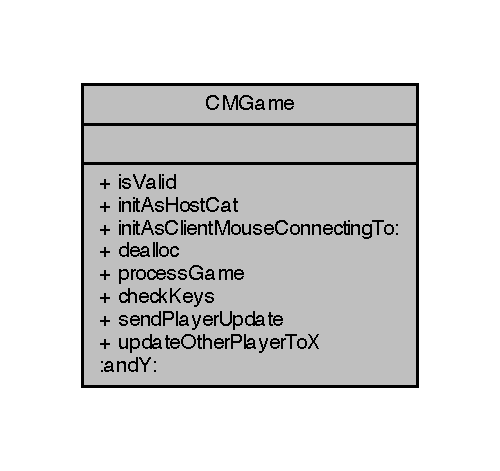
\includegraphics[width=138pt]{class_c_m_game__coll__graph}
\end{center}
\end{figure}


\subsubsection{Detailed Description}
Defines class for the general `game' of the cat and mice. 

\begin{DoxyAuthor}{Author}
Alex Cummaudo 
\end{DoxyAuthor}
\begin{DoxyDate}{Date}
16 Oct 2013 
\end{DoxyDate}


The documentation for this class was generated from the following file\-:\begin{DoxyCompactItemize}
\item 
/\-Users/\-Alex/\-Dropbox/\-Swinburne/\-H\-I\-T2302 -\/ O\-O\-P/\-Projects/\-Cat and Mouse/\#2\-\_\-\-Cat\-Mouse\-\_\-\-Obj\-C\-\_\-\-D\-E\-Coupled/src/{\bf C\-M\-Game.\-h}\end{DoxyCompactItemize}

\subsection{C\-M\-G\-U\-I Class Reference}
\label{interface_c_m_g_u_i}\index{C\-M\-G\-U\-I@{C\-M\-G\-U\-I}}


{\ttfamily \#import $<$C\-M\-G\-U\-I.\-h$>$}



Inheritance diagram for C\-M\-G\-U\-I\-:
\nopagebreak
\begin{figure}[H]
\begin{center}
\leavevmode
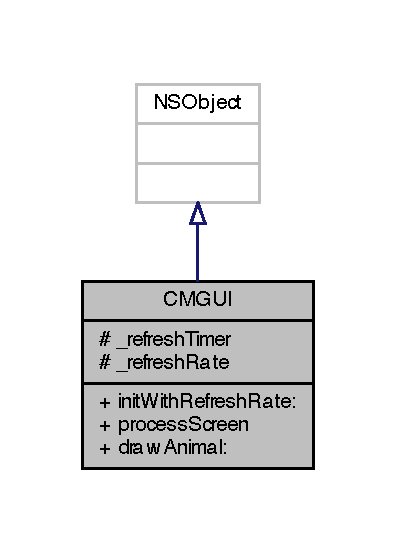
\includegraphics[width=268pt]{interface_c_m_g_u_i__inherit__graph}
\end{center}
\end{figure}


Collaboration diagram for C\-M\-G\-U\-I\-:
\nopagebreak
\begin{figure}[H]
\begin{center}
\leavevmode
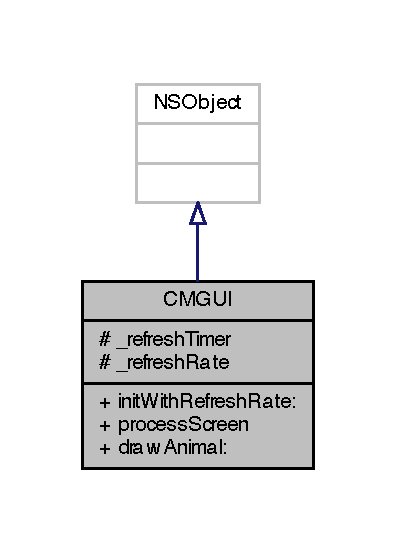
\includegraphics[width=268pt]{interface_c_m_g_u_i__coll__graph}
\end{center}
\end{figure}
\subsubsection*{Instance Methods}
\begin{DoxyCompactItemize}
\item 
(id) -\/ {\bf init\-With\-Refresh\-Rate\-:}
\item 
(void) -\/ {\bf process\-Screen}
\end{DoxyCompactItemize}
\subsubsection*{Protected Attributes}
\begin{DoxyCompactItemize}
\item 
S\-G\-Timer $\ast$ {\bf \-\_\-refresh\-Timer}
\item 
float {\bf \-\_\-refresh\-Rate}
\end{DoxyCompactItemize}


\subsubsection{Detailed Description}
Provides G\-U\-I View for the game to display the game on in a graphics window. 

\begin{DoxyAuthor}{Author}
Alex Cummaudo 
\end{DoxyAuthor}
\begin{DoxyDate}{Date}
22 Oct 2013 
\end{DoxyDate}


\subsubsection{Method Documentation}
\index{C\-M\-G\-U\-I@{C\-M\-G\-U\-I}!init\-With\-Refresh\-Rate\-:@{init\-With\-Refresh\-Rate\-:}}
\index{init\-With\-Refresh\-Rate\-:@{init\-With\-Refresh\-Rate\-:}!CMGUI@{C\-M\-G\-U\-I}}
\paragraph[{init\-With\-Refresh\-Rate\-:}]{\setlength{\rightskip}{0pt plus 5cm}-\/ (id) init\-With\-Refresh\-Rate\-: 
\begin{DoxyParamCaption}
\item[{(float)}]{ref\-Rate}
\end{DoxyParamCaption}
}\label{interface_c_m_g_u_i_ae67dc0a071b5b8d4e6f52c9cdebd81a7}
\index{C\-M\-G\-U\-I@{C\-M\-G\-U\-I}!process\-Screen@{process\-Screen}}
\index{process\-Screen@{process\-Screen}!CMGUI@{C\-M\-G\-U\-I}}
\paragraph[{process\-Screen}]{\setlength{\rightskip}{0pt plus 5cm}-\/ (void) process\-Screen 
\begin{DoxyParamCaption}
{}
\end{DoxyParamCaption}
}\label{interface_c_m_g_u_i_a7978ca9af54ee3ccc9a63eed973a54ea}


\subsubsection{Member Data Documentation}
\index{C\-M\-G\-U\-I@{C\-M\-G\-U\-I}!\-\_\-refresh\-Timer@{\-\_\-refresh\-Timer}}
\index{\-\_\-refresh\-Timer@{\-\_\-refresh\-Timer}!CMGUI@{C\-M\-G\-U\-I}}
\paragraph[{\-\_\-refresh\-Timer}]{\setlength{\rightskip}{0pt plus 5cm}-\/ (S\-G\-Timer$\ast$) \-\_\-refresh\-Timer\hspace{0.3cm}{\ttfamily [protected]}}\label{interface_c_m_g_u_i_a44f086c4978c094f59dc25fb5411b361}
Timer used to refresh the screen at the by clearing the screen and resetting at refresh\-Rate given \index{C\-M\-G\-U\-I@{C\-M\-G\-U\-I}!\-\_\-refresh\-Rate@{\-\_\-refresh\-Rate}}
\index{\-\_\-refresh\-Rate@{\-\_\-refresh\-Rate}!CMGUI@{C\-M\-G\-U\-I}}
\paragraph[{\-\_\-refresh\-Rate}]{\setlength{\rightskip}{0pt plus 5cm}-\/ (float) \-\_\-refresh\-Rate\hspace{0.3cm}{\ttfamily [protected]}}\label{interface_c_m_g_u_i_a1ba9b17e4241db45ccd3ba1086b83adb}


Seconds to refresh the screen at. 



The documentation for this class was generated from the following file\-:\begin{DoxyCompactItemize}
\item 
/\-Users/\-Alex/\-Dropbox/\-Swinburne/\-H\-I\-T2302 -\/ O\-O\-P/\-Projects/\-Cat and Mouse/\#2\-\_\-\-Cat\-Mouse\-\_\-\-Obj\-C\-\_\-\-D\-E\-Coupled/src/{\bf C\-M\-G\-U\-I.\-h}\end{DoxyCompactItemize}

\subsection{C\-M\-Mouse Class Reference}
\label{interface_c_m_mouse}\index{C\-M\-Mouse@{C\-M\-Mouse}}


{\ttfamily \#import $<$C\-M\-Cat\-Mouse.\-h$>$}



Inheritance diagram for C\-M\-Mouse\-:
\nopagebreak
\begin{figure}[H]
\begin{center}
\leavevmode
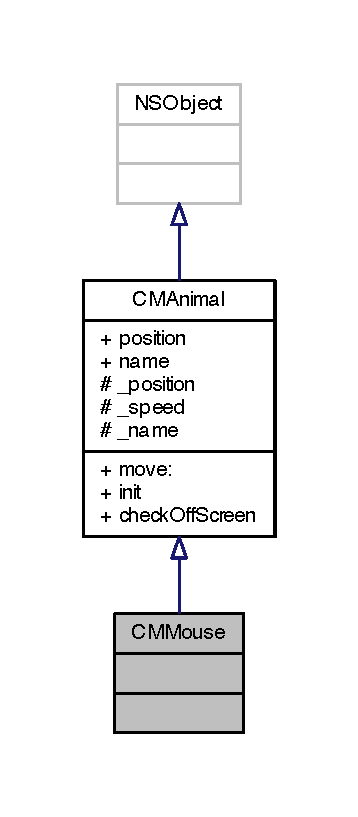
\includegraphics[width=172pt]{interface_c_m_mouse__inherit__graph}
\end{center}
\end{figure}


Collaboration diagram for C\-M\-Mouse\-:
\nopagebreak
\begin{figure}[H]
\begin{center}
\leavevmode
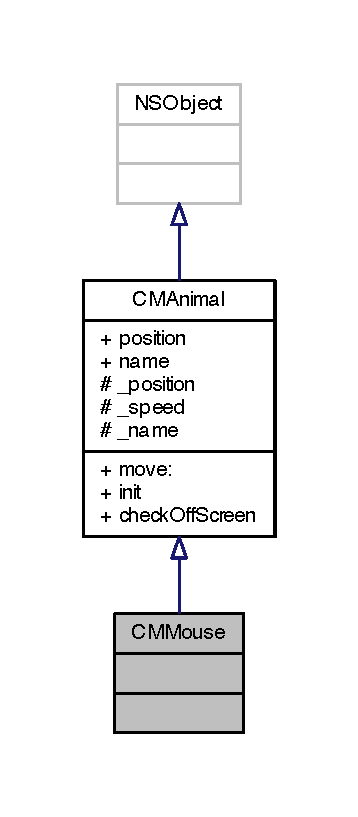
\includegraphics[width=172pt]{interface_c_m_mouse__coll__graph}
\end{center}
\end{figure}
\subsubsection*{Additional Inherited Members}


\subsubsection{Detailed Description}
Defines an class for a playable chasee (i.\-e. the hunted mouse) 

\begin{DoxyAuthor}{Author}
Alex Cummaudo 
\end{DoxyAuthor}
\begin{DoxyDate}{Date}
18 Oct 2013 
\end{DoxyDate}


The documentation for this class was generated from the following file\-:\begin{DoxyCompactItemize}
\item 
/\-Users/\-Alex/\-Dropbox/\-Swinburne/\-H\-I\-T2302 -\/ O\-O\-P/\-Projects/\-Cat and Mouse/\#2\-\_\-\-Cat\-Mouse\-\_\-\-Obj\-C\-\_\-\-D\-E\-Coupled/src/{\bf C\-M\-Cat\-Mouse.\-h}\end{DoxyCompactItemize}

\subsection{C\-M\-Network Class Reference}
\label{interface_c_m_network}\index{C\-M\-Network@{C\-M\-Network}}


{\ttfamily \#import $<$C\-M\-Network.\-h$>$}



Inheritance diagram for C\-M\-Network\-:
\nopagebreak
\begin{figure}[H]
\begin{center}
\leavevmode
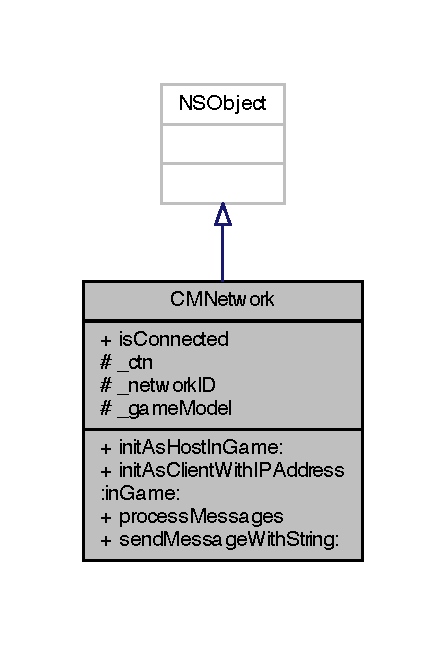
\includegraphics[width=350pt]{interface_c_m_network__inherit__graph}
\end{center}
\end{figure}


Collaboration diagram for C\-M\-Network\-:
\nopagebreak
\begin{figure}[H]
\begin{center}
\leavevmode
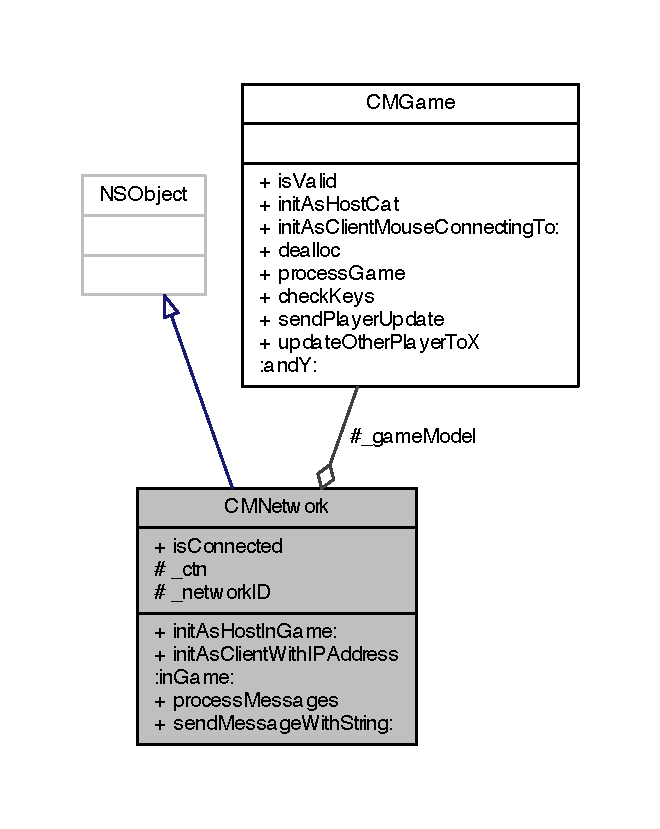
\includegraphics[width=350pt]{interface_c_m_network__coll__graph}
\end{center}
\end{figure}
\subsubsection*{Instance Methods}
\begin{DoxyCompactItemize}
\item 
(id) -\/ {\bf init\-As\-Host}
\item 
(id) -\/ {\bf init\-As\-Client\-With\-I\-P\-Address\-:}
\item 
(void) -\/ {\bf process\-Messages}
\item 
(void) -\/ {\bf dealloc}{\ttfamily  [implementation]}
\item 
(void) -\/ {\bf timeout\-With\-Prompt\-:success\-Message\-:failure\-Message\-:timeout\-Seconds\-:countdown\-Body\-Function\-:break\-Condition\-:}{\ttfamily  [implementation]}
\item 
(S\-G\-Connection $\ast$) -\/ {\bf new\-Connection\-As\-Host}{\ttfamily  [implementation]}
\item 
(S\-G\-Connection $\ast$) -\/ {\bf new\-Connection\-As\-Client\-With\-I\-P\-Address\-:}{\ttfamily  [implementation]}
\item 
(void) -\/ {\bf process\-Event\-:}{\ttfamily  [implementation]}
\item 
(void) -\/ {\bf announce\-Event\-:}{\ttfamily  [implementation]}
\end{DoxyCompactItemize}
\subsubsection*{Protected Attributes}
\begin{DoxyCompactItemize}
\item 
S\-G\-Connection $\ast$ {\bf \-\_\-ctn}
\item 
N\-S\-String $\ast$ {\bf \-\_\-network\-I\-D}
\end{DoxyCompactItemize}
\subsubsection*{Properties}
\begin{DoxyCompactItemize}
\item 
B\-O\-O\-L {\bf is\-Connected}
\end{DoxyCompactItemize}


\subsubsection{Detailed Description}
Packages up data recieved from the controller and passes it to a given network. 

\begin{DoxyAuthor}{Author}
Alex Cummaudo 
\end{DoxyAuthor}
\begin{DoxyDate}{Date}
22 Oct 2013 
\end{DoxyDate}


\subsubsection{Method Documentation}
\index{C\-M\-Network@{C\-M\-Network}!init\-As\-Host@{init\-As\-Host}}
\index{init\-As\-Host@{init\-As\-Host}!CMNetwork@{C\-M\-Network}}
\paragraph[{init\-As\-Host}]{\setlength{\rightskip}{0pt plus 5cm}-\/ (id) init\-As\-Host 
\begin{DoxyParamCaption}
{}
\end{DoxyParamCaption}
}\label{interface_c_m_network_a320a963e841e1a0114ed9c34e3453420}


Constructor initiates a connection as a host. 

\begin{DoxyReturn}{Returns}
The self class pointer 
\end{DoxyReturn}
\index{C\-M\-Network@{C\-M\-Network}!init\-As\-Client\-With\-I\-P\-Address\-:@{init\-As\-Client\-With\-I\-P\-Address\-:}}
\index{init\-As\-Client\-With\-I\-P\-Address\-:@{init\-As\-Client\-With\-I\-P\-Address\-:}!CMNetwork@{C\-M\-Network}}
\paragraph[{init\-As\-Client\-With\-I\-P\-Address\-:}]{\setlength{\rightskip}{0pt plus 5cm}-\/ (id) init\-As\-Client\-With\-I\-P\-Address\-: 
\begin{DoxyParamCaption}
\item[{(N\-S\-String$\ast$)}]{ip\-Addr}
\end{DoxyParamCaption}
}\label{interface_c_m_network_a5da4d088fbf6d0b1ab39179ad85a81b4}


Constructor initiates a connection to a given ip address (as a client) 


\begin{DoxyParams}{Parameters}
{\em ip\-Addr} & The I\-P Address of the host this client will connect to \\
\hline
\end{DoxyParams}
\begin{DoxyReturn}{Returns}
The self class pointer 
\end{DoxyReturn}
\index{C\-M\-Network@{C\-M\-Network}!process\-Messages@{process\-Messages}}
\index{process\-Messages@{process\-Messages}!CMNetwork@{C\-M\-Network}}
\paragraph[{process\-Messages}]{\setlength{\rightskip}{0pt plus 5cm}-\/ (void) process\-Messages 
\begin{DoxyParamCaption}
{}
\end{DoxyParamCaption}
}\label{interface_c_m_network_aa08f5e2e1b9dbcfd21c21d3f1bb0a17a}


Process messages that are being recieved (i.\-e. incoming network string to event) 

\begin{DoxyNote}{Note}
Messages recieved in the format\-: key\-:value,key\-:value, etc. Hence we want to parse the msg back into its event kind
\end{DoxyNote}
\index{C\-M\-Network@{C\-M\-Network}!dealloc@{dealloc}}
\index{dealloc@{dealloc}!CMNetwork@{C\-M\-Network}}
\paragraph[{dealloc}]{\setlength{\rightskip}{0pt plus 5cm}-\/ (void) dealloc 
\begin{DoxyParamCaption}
{}
\end{DoxyParamCaption}
\hspace{0.3cm}{\ttfamily [implementation]}}\label{interface_c_m_network_a20b0186561b122121f42d88f96ecc7c3}


Destructor sends goodbye message and asks \doxyref{C\-M\-Event\-Manager}{p.}{interface_c_m_event_manager} to forget about me and closes all connections. 

\index{C\-M\-Network@{C\-M\-Network}!timeout\-With\-Prompt\-:success\-Message\-:failure\-Message\-:timeout\-Seconds\-:countdown\-Body\-Function\-:break\-Condition\-:@{timeout\-With\-Prompt\-:success\-Message\-:failure\-Message\-:timeout\-Seconds\-:countdown\-Body\-Function\-:break\-Condition\-:}}
\index{timeout\-With\-Prompt\-:success\-Message\-:failure\-Message\-:timeout\-Seconds\-:countdown\-Body\-Function\-:break\-Condition\-:@{timeout\-With\-Prompt\-:success\-Message\-:failure\-Message\-:timeout\-Seconds\-:countdown\-Body\-Function\-:break\-Condition\-:}!CMNetwork@{C\-M\-Network}}
\paragraph[{timeout\-With\-Prompt\-:success\-Message\-:failure\-Message\-:timeout\-Seconds\-:countdown\-Body\-Function\-:break\-Condition\-:}]{\setlength{\rightskip}{0pt plus 5cm}-\/ (void) timeout\-With\-Prompt\-: 
\begin{DoxyParamCaption}
\item[{(N\-S\-String$\ast$)}]{msg\-Prompt}
\item[{successMessage:(N\-S\-String$\ast$)}]{msg\-Suc}
\item[{failureMessage:(N\-S\-String$\ast$)}]{msg\-Fail}
\item[{timeoutSeconds:(int)}]{timeout\-Secs}
\item[{countdownBodyFunction:(void ($^\wedge$)}]{countdown\-Body}
\item[{breakCondition:(B\-O\-O\-L ($^\wedge$)}]{break\-Condition}
\end{DoxyParamCaption}
\hspace{0.3cm}{\ttfamily [implementation]}}\label{interface_c_m_network_a4ada0136c4d624c549abb7593376f5f9}


The timeout connection; runs the passed function success on a success, and error function on error; allow passing of two block objects can be passed in as parameters to the timeout. 


\begin{DoxyParams}{Parameters}
{\em msg\-Prompt} & Prompt message announced when timeout begins (i.\-e., why we're having a timeout). \\
\hline
{\em msg\-Succ} & Message announced when timeout did not run out and the break condition was met \\
\hline
{\em msg\-Fail} & Message announced when timeout did ran out of timeout\-Secs and the break condition was never met \\
\hline
{\em timeout\-Secs} & How long to run timeout for \\
\hline
{\em countdown\-Body} & Function to run every second on timeout \\
\hline
{\em break\-Condition} & Function that returns a bool to check whether or not the timeout should break \\
\hline
\end{DoxyParams}
\index{C\-M\-Network@{C\-M\-Network}!new\-Connection\-As\-Host@{new\-Connection\-As\-Host}}
\index{new\-Connection\-As\-Host@{new\-Connection\-As\-Host}!CMNetwork@{C\-M\-Network}}
\paragraph[{new\-Connection\-As\-Host}]{\setlength{\rightskip}{0pt plus 5cm}-\/ (S\-G\-Connection $\ast$) new\-Connection\-As\-Host 
\begin{DoxyParamCaption}
{}
\end{DoxyParamCaption}
\hspace{0.3cm}{\ttfamily [implementation]}}\label{interface_c_m_network_a70ea6defc2f20045523b267c109a71b2}


Initiates the connection as a host, returning true or false on a success or error. 

\begin{DoxyReturn}{Returns}
A new host connection to work with 
\end{DoxyReturn}
Define new\-Connection as \-\_\-\-\_\-block to allow access to the

Force break condition to be true \index{C\-M\-Network@{C\-M\-Network}!new\-Connection\-As\-Client\-With\-I\-P\-Address\-:@{new\-Connection\-As\-Client\-With\-I\-P\-Address\-:}}
\index{new\-Connection\-As\-Client\-With\-I\-P\-Address\-:@{new\-Connection\-As\-Client\-With\-I\-P\-Address\-:}!CMNetwork@{C\-M\-Network}}
\paragraph[{new\-Connection\-As\-Client\-With\-I\-P\-Address\-:}]{\setlength{\rightskip}{0pt plus 5cm}-\/ (S\-G\-Connection $\ast$) new\-Connection\-As\-Client\-With\-I\-P\-Address\-: 
\begin{DoxyParamCaption}
\item[{(N\-S\-String $\ast$)}]{ip\-Addr}
\end{DoxyParamCaption}
\hspace{0.3cm}{\ttfamily [implementation]}}\label{interface_c_m_network_ad32e2a1d2b2f2c749d4d63cc6627d006}


Initiates the connection as a client, returning true or false on a success or error. 


\begin{DoxyParams}{Parameters}
{\em ip\-Addr} & I\-P Address that this client should connect to \\
\hline
\end{DoxyParams}
\begin{DoxyReturn}{Returns}
A new client connection to work with 
\end{DoxyReturn}
Force break condition to be true \index{C\-M\-Network@{C\-M\-Network}!process\-Event\-:@{process\-Event\-:}}
\index{process\-Event\-:@{process\-Event\-:}!CMNetwork@{C\-M\-Network}}
\paragraph[{process\-Event\-:}]{\setlength{\rightskip}{0pt plus 5cm}-\/ (void) process\-Event\-: 
\begin{DoxyParamCaption}
\item[{({\bf C\-M\-Event} $\ast$)}]{e\-Data}
\end{DoxyParamCaption}
\hspace{0.3cm}{\ttfamily [implementation]}}\label{interface_c_m_network_a79182ec07c3411943efe92aba5fc7586}


Process the event data by packaging it and sending it over the network as a string (i.\-e. an outgoing event to a network string) 


\begin{DoxyParams}{Parameters}
{\em e\-Data} & Event Data to process \\
\hline
\end{DoxyParams}


Reimplemented from {\bf $<$\-C\-M\-Event\-Processor$>$} \doxyref{}{p.}{protocol_c_m_event_processor-p_a2c1a51a02e850b72f7294766f20702f2}.

\index{C\-M\-Network@{C\-M\-Network}!announce\-Event\-:@{announce\-Event\-:}}
\index{announce\-Event\-:@{announce\-Event\-:}!CMNetwork@{C\-M\-Network}}
\paragraph[{announce\-Event\-:}]{\setlength{\rightskip}{0pt plus 5cm}-\/ (void) announce\-Event\-: 
\begin{DoxyParamCaption}
\item[{(N\-S\-String $\ast$)}]{message}
\end{DoxyParamCaption}
\hspace{0.3cm}{\ttfamily [implementation]}}\label{interface_c_m_network_a10a4c149d59fbfd09dc59a2603b8cf90}


Sends an event to all subscribers with the given message. 


\begin{DoxyParams}{Parameters}
{\em message} & Message to announce when creating an Event \\
\hline
\end{DoxyParams}


\subsubsection{Member Data Documentation}
\index{C\-M\-Network@{C\-M\-Network}!\-\_\-ctn@{\-\_\-ctn}}
\index{\-\_\-ctn@{\-\_\-ctn}!CMNetwork@{C\-M\-Network}}
\paragraph[{\-\_\-ctn}]{\setlength{\rightskip}{0pt plus 5cm}-\/ (S\-G\-Connection$\ast$) \-\_\-ctn\hspace{0.3cm}{\ttfamily [protected]}}\label{interface_c_m_network_a0a264da400cb4d9bb8c16cbc66a8908a}


Network connection controller between client and host. 

\index{C\-M\-Network@{C\-M\-Network}!\-\_\-network\-I\-D@{\-\_\-network\-I\-D}}
\index{\-\_\-network\-I\-D@{\-\_\-network\-I\-D}!CMNetwork@{C\-M\-Network}}
\paragraph[{\-\_\-network\-I\-D}]{\setlength{\rightskip}{0pt plus 5cm}-\/ (N\-S\-String$\ast$) \-\_\-network\-I\-D\hspace{0.3cm}{\ttfamily [protected]}}\label{interface_c_m_network_a161ebaba32492602e1c445e76a890e89}


Defines a unique address of this machine. 



\subsubsection{Property Documentation}
\index{C\-M\-Network@{C\-M\-Network}!is\-Connected@{is\-Connected}}
\index{is\-Connected@{is\-Connected}!CMNetwork@{C\-M\-Network}}
\paragraph[{is\-Connected}]{\setlength{\rightskip}{0pt plus 5cm}-\/ (B\-O\-O\-L) is\-Connected\hspace{0.3cm}{\ttfamily [read]}, {\ttfamily [atomic]}, {\ttfamily [assign]}}\label{interface_c_m_network_a70dba80bb8b16b179d3a79fcc4d62786}


Gets connection status. 

\begin{DoxyReturn}{Returns}
Y\-E\-S on a connection with another machine or N\-O when not 
\end{DoxyReturn}


The documentation for this class was generated from the following files\-:\begin{DoxyCompactItemize}
\item 
/\-Users/\-Alex/\-Dropbox/\-Swinburne/\-H\-I\-T2302 -\/ O\-O\-P/\-Projects/\-Cat and Mouse/\#2\-\_\-\-Cat\-Mouse\-\_\-\-Obj\-C\-\_\-\-D\-E\-Coupled/src/{\bf C\-M\-Network.\-h}\item 
/\-Users/\-Alex/\-Dropbox/\-Swinburne/\-H\-I\-T2302 -\/ O\-O\-P/\-Projects/\-Cat and Mouse/\#2\-\_\-\-Cat\-Mouse\-\_\-\-Obj\-C\-\_\-\-D\-E\-Coupled/src/{\bf C\-M\-Network.\-m}\end{DoxyCompactItemize}

\end{document}
